\section{Introduction}
\begin{comment}


\end{comment}

A programmer's mood affects their activities and performance as programming involves various forms of cognitive tasks~\cite{khan2011moods}. 
The collaborative nature of today's software development
means that a developer's mood can be affected by other
developers, and conversely, collaborating developers can be 
affected by one developer's 
mood~\cite{murgia2014developers,graziotin2014happy,curtis1988field}. 
Studies in other domains also show that organizational events can cause affective reactions which in turn influence performance and job satisfaction~\cite{parkinson1996changing}. 

Therefore, software engineering researchers have increasingly studied emotion in software engineering in recent years~\cite{jongeling2017negative}. 
Recent studies involve 
mining software artifacts, 
understanding signals of human emotions hidden in those artifacts, and 
then analyzing the signals in automated ways. 
The findings of these studies could be used by teams to 
track mood and formulate new strategies to ensure 
a healthy environment.


Researchers often use natural language processing tools to capture the emotion in a team.
One place where teams express emotion is on social collaborative sites
like GitHub, where
developers communicate with each other to maintain their projects~\cite{storey2010impact}. 
When developers use these sites, 
researchers can analyze the detailed history of project development, 
as well as developers' communication about the project in the form of issues, for example. 
Such textual artifacts present the opportunity 
to use natural language processing tools 
to do different affect analyses 
for different purposes~\cite{ortu2015bullies,ebert2017confusion,gachechiladze2017anger}. 
While analyzing sentiment is the most commonly used technique to measure emotions, 
researchers have also used natural language tools to measure 
politeness~\cite{ortu2015bullies}, which is an important 
factor in the on-boarding process~\cite{steinmacher2015social}.
Thus, in this paper, we focus on sentiment and 
politeness  analysis tools. 

% maybe ~\cite{montoyo2012subjectivity} somehow? no need
Despite the use of automated tools for analyzing sentiment and 
politeness, significant questions remain about the tools' reliability.
Researchers who focus on sentiment analysis have provided strong data
that the tools are less effective when applied to new domains they 
were not trained on~\cite{novielli2015challenges,gamon2005pulse}. 
In our domain, Jongeling and colleagues have 
shown that different sentiment analysis tools yield different 
results when used on data from a JIRA repository~\cite{jongeling2017negative}. 
%also tools for StackOverflow might not work on issues (for example). no nedd
Hence, understanding the reliability of these tools will help 
software engineering researchers know whether they can use these
tools to reach conclusions confidently.

In this paper, we study the reliability of popular sentiment analysis 
and politeness tools in the context of developer discussions.
To do so, we randomly chose 589 comments from pull requests and issues on GitHub,
manually annotated them for sentiment and politeness using human coders,
and compared those annotations against the results produced by the tools. 

The major contributions of this paper are:
\begin{enumerate}
    \item A benchmark of 589 GitHub comments, 
    hand-rated by humans for sentiment and politeness, 
    \item An annotation scheme that can be used to rate 
    the politeness of comments in discussions, and
    \item A reliability evaluation of six sentiment analysis 
    tools and one politeness tool.
\end{enumerate}

The dataset, coding schemes, and other associated files have been made publicly available at \href{https://tinyurl.com/yabncd7b}{https://tinyurl.com/yabncd7b}.
%todo make the repo public


\section{Related Work}\label{relwork}
%-- give evidence of infinite dimensions of emotions-- not needed
%-- why is github an important domain to look at
\subsection{Sentiment Analysis in Software Engineering}\label{rwsent}

Sentiment analysis focuses on the application of 
classifying texts as to their polarity 
(positive, negative or neutral)~\cite{pang2008opinion}. 
Using data from GitHub, 
Guzman and colleagues applied sentiment analysis 
to study commit comments~\cite{guzman2014sentiment}, 
while Pletea and colleagues tried to find a correlation between security-related discussions and fluctuating sentiments~\cite{pletea2014security}. 
Other platforms, 
including the Gentoo community and Stack Overflow, 
have also been studied to understand developers' 
sentiments~\cite{garcia2013role,islam2016towards,guzman2013towards,novielli2014towards}.

While most of these works have used common tools, 
research on specialized tools for software engineering domain 
is ongoing. 
Customized tools try to overcome the problems 
of the prior common tools 
that were trained on texts 
from unrelated domains 
by having their own sentiment oracle 
for the software engineering domain~\cite{ahmed2017senticr,calefato2017sentiment}. 
However, they have used different or no coding schemes 
while annotating the texts by human raters, 
which might lead them to have subtle differences in their understanding of sentiment in this domain.

\subsection{Politeness in Software Engineering}

Politeness can be described as 
"the practical application of good manners or etiquette"~\cite{wiki:pol}. 
Politeness is a strong factor in social collaborations~\cite{ortu2015would,wang2008politeness}. 
Research is also going on in the software engineering domain 
to study the impact of politeness expressed by developers. 
For example, Ortu and colleagues concluded that 
"the more polite developers were, 
the less time it took to fix an issue", 
while Tsay and colleagues studied GitHub discussions 
and found that, 
"the level of a submitter's prior interaction on a project changed how politely developers discussed the contribution and the nature of proposed alternative solutions"~\cite{ortu2015would,tsay2014let}. However, similar to sentiment analysis, different studies had different methods to rate politeness~\cite{tsay2014let,brownsoftware}.


\subsection{Challenges for Sentiment \& Politeness Analysis in Software Engineering}

Many researchers are planning to study 
the emotional awareness in collaborative software engineering~\cite{dewan2015towards}. 
However, challenges lie in correctly identifying any type of affect before we can use the data for further analysis. 
A recent work explores the possibilities of correctly judging emotions from texts extracted from software engineering platforms~\cite{murgia2014developers}. 
The authors found 
poor to moderate agreement between human raters 
on different types of emotions. 
They conclude that 
``more investigation is needed before 
building a fully automatic emotion mining tool.''
Besides, Novielli and colleagues point towards 
the domain dependency of existing tools 
which makes it harder to apply them in new corpora~\cite{novielli2015challenges}. 

Jongeling and his colleagues have shown 
how different tools lead to different results of sentiment 
in a new data set of JIRA issue reports~\cite{jongeling2017negative}. They also show that ``this disagreement [between different tools] 
can lead to diverging conclusions 
and that previously published results cannot be replicated 
when different sentiment analysis tools are used.'' 
Another work also used existing tools 
on code review comments from Gerrit 
and found a poor performance by the tools~\cite{ahmed2017senticr}. 
We find similar results also in Lin and colleagues' work~\cite{lin2018sentiment}.
This establishes that the reliability tools should be established
before the tool can be used for further analysis.

Just as Jongeling and colleagues 
evaluated the reliability of four sentiment analysis tools, 
we also perform a similar evaluation 
over a new dataset of GitHub comments 
with an addition of two tools 
that are specifically built for the software engineering domain. Moreover, we also extend our evaluation 
towards the reliability of politeness analysis 
on GitHub comments.  
   

\section{Methodology}

Our goal is to evaluate the reliability of sentiment and politeness analysis tools in developer discussions by examining the tools' performance over GitHub comments.
Before we evaluate the reliability of tools for doing affect analysis,
we first need to define our gold standard for evaluation.
Like other works~\cite{calefato2017sentiment,ahmed2017senticr}, we use human coders to create
this gold standard.
However, before taking human ratings at face value, we first ask
to what extent human coders agree with each other:

\begin{itemize}

\item\textbf{RQ1.} How consistent are \emph{human coders} to rate sentiment and politeness on GitHub comments?

\end{itemize}

\noindent
Our next research questions evaluate the tools:

\begin{itemize}

\item\textbf{RQ2.} How reliable are \emph{sentiment analysis tools} on GitHub comments?

\item\textbf{RQ3.} How reliable are \emph{politeness analysis tools} on GitHub comments? 

\end{itemize}

\subsection{Data Collection \& Manual Raters}\label{data}

% % There are many ways for a developer to put comments in GitHub, e.g. commit comments, comments in pull request review and issue discussion boards. However, while commit comments may contain texts for documentation purpose; pull request review and issue comments are mostly discussion between developers. Hence, the later is a more standard metric of interaction between developers. In our study, we only evaluate comments from pull request review and issue section in GitHub.
% under pull request review and issue section
We chose GitHub as our research setting 
because it is the largest code host 
in the world~\cite{gousios2014lean}. 
The GitHub  documentation designates 
issue and pull request sections 
as the appropriate place for 
both general and specific project discussion
 between developers.\footnote{\url{https://guides.github.com/features/issues/}}
 Hence, we chose comments from these discussion threads 
 to evaluate our tools on. 

% We chose comments from GitHub because it is the largest code host in 
% the world~\cite{gousios2014lean}, and is regularly used in software 
% engineering studies. Because the GitHub documentation designates
% issue and pull request sections as the appropriate place for both general and specific project discussion between developers, we investigated these discussion threads for our test corpus.

To get the comments, 
we use the GHTorrent project.\footnote{http://ghtorrent.org/} 
However, while GHTorrent does archive code-review comments, 
it does not contain the general discussion comments 
under issues and pull requests. 
Furthermore, 
GitHub comments may contain code snippets.
%many of the comments that GHTorrent does have 
%contain code snippets that affect analyzers cannot correctly process. 
To remove those code snippets, 
we need to be able to detect the HTML tags around the code, 
assuming that the authors highlighted them. 
For these purposes, 
we augment our data by mining GitHub's web pages 
to acquire the comments from the issue and pull request review sections. 
This way, we can also get the HTML tags.

As manual annotation is a time-consuming task, 
we estimated 
every hundred comments 
would take one hour to complete by one person. 
For each comment, 
we would have two human coders to 
manually go through and annotate, 
as a previous study found that 
"having more than two raters 
does not change 
the agreement significantly"~\cite{murgia2014developers}. 
We estimated that annotation of 600 comments 
can be completed within reasonable time and effort.
Adding 40 comments more as a cautionary step, 
we randomly picked 640 comments 
from all the public projects from the data we collected.
To estimate how much these comments
represent developer discussions,
We randomly picked 
20 comments out of these 640 
and manually investigated their origins.
All 20 comments came from different projects 
and the projects appear to represent valid software development.
18 out of these 20 projects have a clear description 
of the project in their README files.
Out of these 20 projects, 
4 projects had only 1 contributor, 
3 projects had 2 contributors, 
and 1 project had 4 contributors.
The remainder of the 12 projects had at least 15 contributors.

During pre-inspection, 
we had to remove 51 comments as they were 
either incomplete fragments, 
duplicates, 
code snippets without commentary, 
non-English statements, 
or parts of discussions that are no longer available 
(due to, for example, invalid URLs). 
The rationale behind the last factor is that 
if the coders want to see the whole discussion 
of which a comment belongs to
in order to have an understanding 
of the underlying context, 
they wouldn't be able to do so. 
We provide the final 589 comments to the human coders 
removing only the HTML tags. 
However, before feeding these comments to the tools, 
we also remove the code snippets and URLs, 
as they would get incorrectly processed by the tool,
which
wrongly considers them English texts 
and hence may bias the result. 
The raters were also provided with the URL of the webpage 
containing the comment.
Also, while we kept emoticons in the comments, 
we had to strip out the emojis 
before providing the comments 
to the human coders and the tools.
The emojis in the GitHub comments 
are stored images 
that get fetched from a central hosting location.
While we could replace the emojis 
by their titles using the images' HTML tags, 
the tools would have been unable to detect them, 
as they are not trained in this way.
So we removed all the emojis 
from the comments in our test data.

While the first coder (Coder 1) rated all the comments, 
we had two other coders 
who went through half of the data set each individually. 
All the coders were graduate and undergraduate students 
of the Computer Science department. 
We provided a coding guideline 
to the raters before providing the comments, 
explained in Sections~\ref{sentscheme} and~\ref{polscheme}. 
The human coders had a short practice set 
consisting of 10 sample comments 
before starting with the main data set.

After the first iteration, 
where everybody separately annotated the texts, 
Coder 1 sat with each of the other coders 
to discuss the comments they disagreed on 
and their rationale behind their rating. 
This resulted in reaching consensus 
for the initially disputed comments 
and bringing out insights over our coding guidelines.



\begin{comment}
 and try to determine if they give satisfactory results on GitHub comments. This leads to our first research question,
\newline
\newline
\textbf{RQ1 - How do popular sentiment analysis tools fare on real-life GitHub comments?}
\newline
\newline
 Thus leading us to our second research question,
\newline
\newline
\textbf{RQ2: How does popular politeness analysis tool fare on real-life GitHub comments? }
\newline
\newline
\end{comment}


\subsection{Sentiment Annotation Scheme}\label{sentscheme}


As mentioned in Section~\ref{rwsent}, 
previous work has used different or no coding schemes 
while doing sentiment rating in the software engineering domain. 
To not deviate a lot from the previous works, 
but still giving our coders a basic set of strategies, 
we make use of the simple annotation scheme 
from a prior work developed by Mohammad~\cite{mohammad2016practical}. 
Based on this scheme, 
the raters were asked to label each comment as 
either positive, negative, neutral, mixed or sarcasm. 
The "mixed" here stands for a text containing both types of emotions. Our tools label texts as "neutral" 
where opposite emotions counter each other. 
From that perspective, 
we eventually classified the texts as "neutral" 
which were given a "mixed" rating by the human raters. 
We omitted the texts rated "sarcasm" by the human raters 
from our test data as there is no clear guideline 
on how to match its label with the 
possible ratings the tools have as output. 

\subsection{Politeness Annotation Scheme}\label{polscheme}

We could not find any commonly used politeness scheme 
to rate textual documents. 
So, we developed and began with an experimental coding scheme\footnote{https://tinyurl.com/ycts7vhr} 
based on the work of 
Brown and Levinson's politeness theory~\cite{brown1987politeness} 
and Culpeper's work of impoliteness~\cite{culpeper1996towards}. 
From these theories, 
we select the strategies that are relevant to written communication (filtering out the non-verbal cues of politeness). 
The strategies depend on the theory of "face", 
where positive face points towards the desire 
to be liked or appreciated or approved etc. 
and negative face is the desire 
to not to be imposed upon, intruded, or otherwise put upon.

\FloatBarrier
\begin{table}[H]
	\centering
	\caption{Coding Strategies for Politeness}
	\label{poltable}
	% \begin{threeparttable}
	\begin{tabular}{ | m{1.75cm} | m{2cm}|| m{2cm} | m{1.75cm} | }
		\hline
		\multicolumn{2}{|c||}{Politeness} & \multicolumn{2}{c|}{Impoliteness} \\
		\hline
		Strategies & Examples & Strategies & Examples \\ 
		\hline
		Positive Politeness: Helping hearer's positive face  & Gratitude: "I really appreciate it" & Positive Impoliteness: threatening hearer's positive face & Seeking disagreement: "I don't agree with this style of coding" \\
		\hline
		Negative Politeness: Helping hearer's negative face & Use of Verbal Hedges: "I suggest we write it this way" & Negative Impoliteness: threatening hearer's negative face  & Direct accusation: "You made these faulty changes"\\
		\hline
		Indirect Politeness: Offering advice through indirect implication & "It's really cold here" could imply a request to shut the window down & Sarcasm or Mock Politeness & Having sarcastic tone: "static??? really???" \\
		\hline
		\multicolumn{2}{c|}{--} & Withhold Politeness:\tablefootnote{Excluded in the modified scheme after the experiment} Absence of politeness where it is expected & Depends on context: Failing to thank somebody after help\\
		\cline{3-4}
		% \begin{tablenotes}
		% % \item[1] Excluded in the modified scheme after the experiment
		% \end{tablenotes}
	\end{tabular}
	% \end{threeparttable}
	%\footnotetext{Excluded in the modified scheme after the experiment}
\end{table}

However, this being an experimental coding scheme, 
the raters were given the web page 
of the discussion thread containing the comment 
and were encouraged to dive 
into the detail of the context of the whole conversation 
and use their own judgment while rating. 
Additionally, they were asked to give remarks 
if they found any criterion 
that are not covered by the scheme 
or a strategy in the scheme that
do not align with the comment. 
The major criteria of our initial coding scheme 
are shown in Table~\ref{poltable}, along with examples.
Based on this scheme, 
the coders were asked to rate each text as 
very polite, polite, neutral, impolite, and very impolite.
To measure the degree of politeness/impoliteness, 
the coders were suggested to consider 
the frequency of strategies used in the comment 
according to the scheme 
alongside their own judgment and the underlying context.

As mentioned in Section~\ref{data}, 
after the first iteration of rating, 
the Coder 1 had a discussion with the other coders 
about judging criteria 
and reaching a conclusion about the disputed comments. 
Upon the discussion, 
we also modify our coding scheme and 
propose a complete and final one 
which is presented in Section \ref{finalpolscheme}. 
From the discussion, 
the coders also agreed that the initial coding scheme 
was not very clear on how to distinguish 
between the degrees of politeness/impoliteness, 
hence we got varying judgment on them. 
For the purpose of this study, 
we, therefore, merged 
"very polite" and "polite" into one single"polite" group,  
and "very impolite" and "impolite" into an "impolite" group.

\subsection{Tool Selection}
Sentiment analysis is an active field of research 
%in the past decade 
and also possesses commercial interest. 
Hence there are a lot of tools available. 
Jongeling and colleagues point out four tools 
as the most commonly used for sentiment analysis 
across all the domains 
including software engineering research 
(SentiStrength, NLTK, Alchemy, Stanford NLP).
These tools, however, 
are trained on corpora 
that are not related to software engineering.
Therefore, we take two other tools that have been trained on a dataset relevant to developer discussions (Senit4SD, SentiCR). 
% We also take another tool from a recent paper, Senti4SD~\cite{calefato2017sentiment}, into consideration as it is claimed to be "specifically trained to support sentiment analysis in developers' communication channels". We select these 5 tools as popular sentiment analysis tools.
\newline
\indent \textbf{SentiStrength:} Thelwall and colleagues' SentiStrength~\cite{thelwall2010sentiment} 
was developed based on MySpace comments 
and has a ``word strength list'' 
at the core of its algorithm. 
The tool has been frequently used in software engineering research~\cite{garcia2013role,guzman2014sentiment,novielli2015challenges,guzman2013towards,sinha2016analyzing}. 
SentiStrength assigns 
an integer value between 1 to 5 for positive sentiment 
and -1 to -5 for negative sentiment. 
We add both the rating for a text, 
and identify "positive" sentiment if the sum is greater than zero, "negative" if less than zero 
and "neutral" otherwise. 
This interpretation was used in Jongeling's work~\cite{jongeling2017negative}.
\newline
\indent\textbf{Alchemy:} IBM's Alchemy 
provides a text-processing API 
which returns a label for sentiment 
(positive/neutral/negative). 
\newline
\indent\textbf{NLTK:} Bird and colleagues' NLTK~\cite{bird2009natural}, 
which uses multiple corpora in its development, 
has also been used in previous works 
in the software engineering domain~\cite{pletea2014security,rousinopoulos2014sentiment}. 
We use an API provided in \href{www.text-processing.com}{www.text-processing.com} 
to use this tool. 
For each text, it also returns a sentiment label
(positive/neutral/negative).
\newline
\indent\textbf{Stanford NLP:} Socher and colleagues' Stanford NLP 
divides the text into sentences, 
and performs a more advanced grammatical evaluation 
on each sentence 
by generating a sentiment treebank 
through Recursive Neural Tensor Networks~\cite{socher2013recursive}.
It was trained on movie review excerpts 
from the \url{rottentomatoes.com} website. 
It returns an integer score for each sentence 
(0 for neutral, 1 for positive, -1 for negative) 
indicating its sentiment label. 
We rate a text under "positive" or "negative" 
based on the category that has greater number of sentences 
and "neutral" otherwise. 
This approach is similar to that of SentiStrength.
\newline
\indent\textbf{Senti4SD:} This tool, 
developed by Calefato and colleagues~\cite{calefato2017sentiment}, classifies each text by labeling sentiment 
as positive, negative or neutral.
The tool was built using 
questions, answers and comments 
from StackOverflow as its training data. 
\newline
\indent \textbf{SentiCR:} Ahmed and colleagues' SentiCR~\cite{ahmed2017senticr} 
is trained on a dataset 
that comprises of 
code review comments from Gerrit and 
two other datasets developed 
in prior work~\cite{calefato2017sentiment,ortu2016emotional} 
using supervised learning techniques. 
Based on the oracle, 
the tool also return a sentiment label 
for a text 
(positive, neutral and negative).
\newline
\newline
For politeness analysis, we use a tool developed by Danescu-Nicu\-lescu-Mizil and colleagues~\cite{danescu2013computational}. 
While the tool was trained on short texts 
that represent requests/questions, 
the tool identifies general patterns of politeness 
in written texts and 
has been used in recent software engineering studies.
Ortu and colleagues have used this tool 
over a dataset collected from 
the Apache Software Foundation Issue Tracking system, 
a JIRA repository~\cite{ortu2015would,ortu2015bullies}. 
They also show that sentiment and politeness 
are independent metrics having a weak correlation~\cite{ortu2015bullies}. 
As the tool does not have any distinct name, 
we will simply call it the "politeness tool". 

\textbf{Politeness tool:} This tool~\cite{danescu2013computational} tries to measure politeness based on 
"domain-independent lexical and syntactic features 
operationalizing key components of politeness theory, 
such as indirection, deference, impersonalization and modality". 
It was trained and tested 
on different corpora (Wikipedia and Stack Exchange) 
and hence has the claim of being domain independent. 
The tool ``predicts a politeness score between 0 to 1'' 
for each text.   

 
\section{Results}

\subsection{RQ1 }\label{gt}

In the first iteration, 
we had each comment rated by two coders individually 
on both sentiment and politeness. 
If for any comment, 
two coders agreed about the rating, 
we finalized that label for the comment. 
This resulted in 374 comments for politeness 
and 285 comments for sentiment. 
We call this the first set of data as the "agreed" set.
In the second iteration, 
the Coder 1 had a discussion 
with each of the two other human coders. 
From this discussion, 
a conclusive rating was achieved 
for each of the initially disputed comments. 
This resulted in the "final" data set 
containing the newly negotiated ones along with the agreed ones. 
This procedure aligns with a previous paper~\cite{ahmed2017senticr}. Also, during this discussion, 
some insights about how the comments should be rated 
both on "politeness" and "sentiment" were noted. 
These findings have been presented in Sections \ref{finalpolscheme} and \ref{sentschemedis}.
We used both the initially agreed and final set of data 
to evaluate our tools for RQ2 and RQ3. 
The amount of test data is comparable 
with the data set of a previous study 
which took 265 labeled texts to 
perform the evaluation of sentiment analysis tools~\cite{jongeling2017negative}.

%As mentioned before, all of the 589 comments were annotated by the Coder 1, and two other coders annotated one half of the dataset each.
Table \ref{interrater} shows the inter-rater agreement
during manual rating. 
We used Weighted Cohen's Kappa 
because our classes in both of the ratings 
have an implicit ordering. 
When two coders labeled different polarity 
for their ratings 
(positive vs negative and polite vs impolite), 
we counted it as a strong disagreement (weight=2). 
And when one of the labels was neutral, 
and other was a polar one, 
we counted it as a weak disagreement (weight=1).
Coder 1 had a fair and moderate agreement 
with one of the coders (Coder 2) 
for sentiment and politeness respectively and 
fair with the other coder (Coder 3) for both the ratings 
(according to magnitude guidelines presented by Landis and Koch~\cite{landis1977measurement}). 
This agreement rate is similar to what 
Murgia and colleagues found in their work 
for emotions like love, sadness, fear, and joy~\cite{murgia2014developers} and 
points towards the subjectivity of these affects.
However, 
Coder 1's agreement with both the other coders
on politeness 
is higher than on sentiment. 
One reason behind this can be 
that the annotation scheme for politeness 
provided to the coders 
was more detailed with relevant examples 
than the simple scheme for sentiment. 

\vspace{3mm}
\noindent\fbox{%
    \parbox{\linewidth}{%
       \textbf{The $\kappa=.27$ to $.48$ agreement suggests that even human ratings had low sentiment and politeness consistency on GitHub comments.}
    }%
}
\vspace{3mm}


\begin{table}
\centering
\caption{Inter-rater Agreement (Weighted Cohen's Kappa)}
  \label{interrater}
  \begin{tabular}{|c|c|l|}
    \toprule
    Weighted $\kappa$ & Coder 1 and Coder 2 &  Coder 2 and  Coder 3\\
    \midrule
    Sentiment & .38 & .27 \\
    \hline
    Politeness & .48 & .36\\
  \bottomrule
\end{tabular}
\end{table}

% The author then sat with each of the other coder to discuss about the disagreed comments. Then upon discussion, the raters came for a final rating for all of the comments. now pos was , neg was and neu. similarly pol, neu and impolite was . The raters also discussed the reason behind choosing the final rating for them and how the annotation scheme should be modified or added to improve.
While we had substantial amount of disagreement 
between the coders in the first iteration 
and hence found the inconsistency of human rating, 
the coders reached a conclusion for the disputed comments 
through discussion afterwards. 
This way, we completed a data set of comments 
that are hand-rated by humans and 
use it as a benchmark for our evaluation in RQ2 and RQ3.

\subsection{RQ2}
The initially agreed dataset contained 
66 positives, 20 negatives, 198 neutral and 1 sarcasm 
out of total 285 comments. 
And for the final dataset, 
we got 93 positives, 73 negatives, 419 neutral and 4 sarcasm 
out of 589 comments. 
As our dataset is heavily "neutral" biased, 
only F-measures for the tools would be a misleading metric 
as the agreement by chance would be high. 
So, we also calculated Weighted Cohen's Kappa as before, 
to compare the tools' output with the final human ratings. 
We got an output for each comment by all the tools except Alchemy, which failed to give an output for 46 and 70 comments respectively for the agreed and the final data set. 
For the first set of agreed data in Table \ref{sentfirst}, 
Senti4SD turned out to have the best performance among the tools. 
One point to note from the results is 
the relatively low F-measures with a low recall 
of negative comments 
for all the tools compared to 
neutral and positive comments. 
This confirms the "negative bias" of the existing tools, 
that is the misclassification of neutral technical texts 
as emotionally negative~\cite{blaz2016sentiment,novielli2015challenges,calefato2017sentiment}.
In Table \ref{sentfinal}, we show the results 
when we compare the tools with the final dataset. 
In this step, 
we see a major drop in the performance 
of all the tools 
except for SentiCR
and a similar pattern of negative comments 
still doing worse.
The performance drop may indicate
that the initially disputed comments
are harder to rate.
%and there remain subtle aspects of subjectivity in these comments. 
However, the tools' performance 
over both the dataset 
tells us about their overall unreliability.


\vspace{3mm}
\noindent\fbox{%
    \parbox{\linewidth}{%
       \textbf{The $\kappa=.16$ to $.33$ agreement suggests that tools had low sentiment reliability on GitHub comments.}
    }%
}

\begin{table}
\centering
\caption{Performance of Sentiment Analysis Tools for the First Set of  Agreed Data}
\label{sentfirst}
\begin{tabular}{|c|c|c|c|c|}
\hline
\multicolumn{2}{|c|}{ } & \multicolumn{3}{c|}{ F-measure } \\
\hline
tools & Weighted $\kappa$ & neutral & positive & negative \\
\hline
SentiStrength & 0.44 & 74.58\% & 61.54\% & 40.68\% \\
\hline
NLTK & 0.27 & 52.63\% & 55.42\% & 23.73\% \\
\hline
Alchemy & 0.33 & 58.78\% & 58.21\% & 32.65\% \\
\hline
Stanford NLP & 0.26 & 55.85\% & 59.83\% & 19.44\% \\
\hline
Senti4SD & 0.53 & 84.92\% & 68.18\% & 41.03\% \\
\hline
SentiCR & 0.13 & 57.04\% & 29.70\% & 29.91\% \\
\hline
\end{tabular}
\end{table}

\begin{table}
\centering
\caption{Performance of Sentiment Analysis Tools for the Final Set of Data}
\label{sentfinal}
\begin{tabular}{|c|c|c|c|c|}
\hline
\multicolumn{2}{|c|}{ } & \multicolumn{3}{c|}{ F-measure } \\
\hline
tools & Weighted $\kappa$ & neutral & positive & negative \\
\hline
SentiStrength & 0.24 & 65.68\% & 43.01\% & 30.85\% \\
\hline
NLTK & 0.24 & 45.38\% & 45.26\% & 33.86\% \\
\hline
Alchemy & 0.23 & 51.56\% & 41.67\% & 34.48\% \\
\hline
Stanford NLP & 0.16 & 43.05\% & 45.09\% & 26.41\% \\
\hline
Senti4SD & 0.33 & 79.04\% & 50.47\% &  31.25\% \\
\hline
SentiCR & 0.24 & 64.87\% & 43.48\% & 31.02\% \\
\hline
\end{tabular}
\end{table}

\subsection{RQ3}

For politeness, 
the initially agreed dataset contained 
153 polite, 21 impolite and 200 neutral 
out of 374 comments 
while the final dataset contained 
221 polite, 46 impolite and 322 neutral 
out of 589 comments. 
As the politeness tool
gives a score between 0 to 1 
for each text for its politeness, 
we have to first select a threshold 
where we can separate the polite, impolite and neutral comments. 
Over the first data set, we calculated F-measures 
at every .01 interval within the 0--1 range. 
We found the highest F-measure 
being 69.61\%  for polite at a .57 threshold 
and 77.05\% for neutral at a .65 threshold. 
So, intuitively the ideal threshold 
to separate polite vs neutral 
would fall somewhere between that range. 
Our results align with the findings of Jongeling and colleagues,
who found this threshold to be at .611. 
So, we use this threshold and 
rate all those comments as "polite" 
for which the tool gives a higher rating than .611.

However, we found 
very poor results
for impolite comments 
as F-measures at all the ranges were below 20\%. 
Thus, we concluded that 
the tool has low reliability 
in deciding if a comment in our data set is impolite or not. 
Therefore, we decided to merge the "neutral" and "impolite"
into one single class that is "non-polite". 
Thus, eventually, we use the tool 
for a binary classification of the texts 
between polite and non-polite.
We use both the agreed and final data set
to evaluate the single tool. 
Similar to RQ1, 
we use Cohen's kappa (unweighted) and F-measures as our metrics. Table \ref{polresult} shows that this tool also 
has "moderate" agreement over the first agreed data set 
while a "fair" agreement over the final data set. 

\vspace{3mm}
\noindent\fbox{%
    \parbox{\linewidth}{%
       \textbf{The $\kappa=.39$ agreement suggests that the tool had low politeness reliability on GitHub comments.}
    }%
}

\begin{table}
\centering
\caption{Performance of Politeness Analysis tool}
\label{polresult}
\begin{tabular}{|c|c|c|c|c|c|}
\hline
\multicolumn{3}{|c|}{ First Data set }& \multicolumn{3}{c|}{ Final Data set } \\
\hline
 & \multicolumn{2}{c|}{ F-measure } & & \multicolumn{2}{c|}{ F-measure } \\
 \hline
$\kappa$ & polite & neutral & $\kappa$ & polite & neutral \\
\hline
.49 & 67.15\% & 75.94\% & .39 & 60.24\% & 78.37\%\\
\hline
\end{tabular}
\end{table}

\section{Discussion}
\subsection{Final Politeness Coding Scheme} \label{finalpolscheme}

The coders discussed and then changed 
the initial politeness coding scheme. 
We differentiated between implicit politeness 
and \textbf{explicit markers} of politeness 
within a text. 
For example, one coder rated a comment polite 
if he felt that the commenter is giving a detailed explanation 
of something and 
hence putting more effort into the communication. 
All the coders agreed that 
this is an implicit form of politeness. 
Another example would be the fourth strategy of impoliteness 
in our initial coding scheme which 
marks the absence of politeness where it is expected 
as a form of impoliteness. 
All the coders agreed that 
these are the implicit forms of politeness/impoliteness 
and cannot be clearly derived from a single comment 
without knowing the whole underlying context. 
Whereas, other strategies involve "explicit markers" 
like verbal hedges, indirection, and use of positive lexicons. 
So for the comments that were initially disputed, 
we only counted those as `polite' 
which have an explicit marker of politeness 
within the text itself.

Based on our discussion, 
we fully develop a coding scheme
which has less ambiguous steps to detect politeness. 
We also give direction on 
how to rate the degree of politeness/impoliteness 
and what to do with the mixed comments. 
Although we did not use this final modified scheme in our work, 
we hope that this scheme will come useful in future works 
and help in maintaining a clear set of standards 
in rating politeness for texts found in online conversations. 
The scheme is also publicly available at \href{https://tinyurl.com/y8g3b8zn}{https://tinyurl.com/y8g3b8zn}.

\subsection{Insights on Sentiment Coding}\label{sentschemedis}
The main confusion 
while rating the sentiment
came from how to rate the statements of technical details 
containing \textit{bug reports} or \textit{bug fixes} 
(e.g. "fixed", "done") 
which are commonplace in software engineering and 
don't necessarily express an emotion. 
One coder initially rated all texts indicating bug fixes 
as positive 
as these comments mark positive results. 
However, the other coder rated the same texts as neutral 
unless they are explicitly emotive. 
Similar confusion arose with bug reports or crash reports. 
Upon discussion, the coders agreed that 
these texts are samples of normal day-to-day technical details 
in a software project. 
The coders reached a consensus 
that if a text doesn't explicitly show an emotion, 
we would rate it as neutral. 
%The initially disputed comments were resolved on such conclusions. 
This confusion points 
to the necessity of a customized annotation scheme 
for software engineering. 

\subsection{Tools' failure: Case analysis}
%To pinpoint the weaknesses in automated rating, we looked at the comments where the tools had a different rating from the humans.  For the sentiment analysis tools, we perform a case study on Senti4SD, which had the best performance.
 
To investigate why the tools had poor results, 
we looked at the comments where
Senti4SD and the politeness tool
gave different ratings than the humans.
For many lexicons, 
Senti4SD might not have the accurate weight 
and hence inaccurately give a polar rating. 
Some common words like "error", "wrong" or "problem" 
have been rated as negative by the tool 
while the human raters found them neutral. 
There are also cases when the tool gave a neutral rating 
but humans found some pole of emotion. 
For example, the tool might not have an adequate weight 
for words like "thanks", "congrats", "LGTM" 
and the emoticons which human raters found 
as signs of positive sentiment. 
The tool could also not catch 
subtle criticism or frustration in the comments and 
failed on very short texts like 
"Yikes" and "Sorry". 
Again, for the texts containing mixed sentiments, 
the tool could not appropriately find 
the eventual intention of the commenter. 
Other sentiment analysis tools did not 
exactly have the same points of differences 
and had varying precision and recall over all the classes. 
%The rationale behind this discrepancy is that different tools had different training data and therefore had different weights to different judging criteria. This also shows us the need of having a standard annotation scheme for software engineering domain, and train a tool based on that.

For the politeness tool, 
there are a lot of samples 
which went marginally wrong 
judging by the score that the tool provided for them.
Similar to Senti4SD, the tools have problems
on short texts and
with proper lexicon weights. 
The failure for impolite comments is because 
impoliteness is much more subtle within the context. 
Also, even for some explicit syntactic features, 
like direct orders (e.g. "Do not add", "see above", "replace") 
came out as neutral by the tool. 
However, having distinct cases of failures for these tools 
suggests improvement is possible.

\section{Threats to Validity}
One major threat of our study is 
that we only had two human coders 
per each comment. 
Given by the subjectivity of such analysis, 
more coders could ensure more reliable human evaluation.
Also, we had one coder rating all the comments 
and two other rating half of the data set each.
This creates a possibility of human bias 
in our manual rating.
However, we also present the results over the comments 
for which both the coders agree on the label 
without having a prior discussion.
Besides this, Danescu-Niculescu-Mizil and his colleagues 
for their politeness tool used Brown and Levinson's theory 
to extract features of politeness out of the data 
that were manually rated. 
Our coding scheme is also based on the same politeness theory. 
This biases our annotation of the comments 
towards the tool's internal workings. 
%If we had a different or no coding scheme during the rating, the performance of the politeness with respect to the human rating could have come out worse. 
Also, 
we removed the URLs 
before feeding the comments to the tool 
but 
not from the comments provided to the coders 
which creates a difference between the inputs.
%However, 
%the human coders did not take the URLs into account 
%as they are not commentary texts.
Finally, while we randomly picked 589 comments, they may not be representative of the whole GitHub community.

\section{Conclusion}
Studying the emotions expressed by the developers
is a fertile ground for research. 
However, we find that 
not only the popular existing tools are unreliable,
even humans too are inconsistent  
in identifying sentiment and politeness 
in developer discussions.
This demonstrates the need for 
standardized coding schemes 
for the human coders
in order to build an oracle
and then perform customized training 
on the tools
to perform reliable affect analysis
in the software engineering domain. 

%Through these conclusions, we demonstrate the need for a standard and more concrete definition of affects and their coding schemes to develop a reliable ground truth for affect analysis and train customized tools for the software engineering domain.  

\section*{Acknowledgements}

Thanks to the Developer Liberation Front and anonymous
reviewers for their helpful suggestions.
This material is based in part upon work supported by the 
National Science Foundation under grant number 1252995.



\begin{comment}
\subsection{Citations}
Citations to articles~\cite{bowman:reasoning,
clark:pct, braams:babel, herlihy:methodology},
conference proceedings~\cite{clark:pct} or maybe
books \cite{Lamport:LaTeX, salas:calculus} listed
in the Bibliography section of your
article will occur throughout the text of your article.
You should use BibTeX to automatically produce this bibliography;
you simply need to insert one of several citation commands with
a key of the item cited in the proper location in
the \texttt{.tex} file~\cite{Lamport:LaTeX}.
The key is a short reference you invent to uniquely
identify each work; in this sample document, the key is
the first author's surname and a
word from the title.  This identifying key is included
with each item in the \texttt{.bib} file for your article.

The details of the construction of the \texttt{.bib} file
are beyond the scope of this sample document, but more
information can be found in the \textit{Author's Guide},
and exhaustive details in the \textit{\LaTeX\ User's
Guide} by Lamport~\shortcite{Lamport:LaTeX}.

This article shows only the plainest form
of the citation command, using \texttt{{\char'134}cite}.

Some examples.  A paginated journal article \cite{Abril07}, an enumerated
journal article \cite{Cohen07}, a reference to an entire issue \cite{JCohen96},
a monograph (whole book) \cite{Kosiur01}, a monograph/whole book in a series (see 2a in spec. document)
\cite{Harel79}, a divisible-book such as an anthology or compilation \cite{Editor00}
followed by the same example, however we only output the series if the volume number is given
\cite{Editor00a} (so Editor00a's series should NOT be present since it has no vol. no.),
a chapter in a divisible book \cite{Spector90}, a chapter in a divisible book
in a series \cite{Douglass98}, a multi-volume work as book \cite{Knuth97},
an article in a proceedings (of a conference, symposium, workshop for example)
(paginated proceedings article) \cite{Andler79}, a proceedings article
with all possible elements \cite{Smith10}, an example of an enumerated
proceedings article \cite{VanGundy07},
an informally published work \cite{Harel78}, a doctoral dissertation \cite{Clarkson85},
a master's thesis: \cite{anisi03}, an online document / world wide web
resource \cite{Thornburg01, Ablamowicz07, Poker06}, a video game (Case 1) \cite{Obama08} and (Case 2) \cite{Novak03}
and \cite{Lee05} and (Case 3) a patent \cite{JoeScientist001},
work accepted for publication \cite{rous08}, 'YYYYb'-test for prolific author
\cite{SaeediMEJ10} and \cite{SaeediJETC10}. Other cites might contain
'duplicate' DOI and URLs (some SIAM articles) \cite{Kirschmer:2010:AEI:1958016.1958018}.
Boris / Barbara Beeton: multi-volume works as books
\cite{MR781536} and \cite{MR781537}.

A couple of citations with DOIs: \cite{2004:ITE:1009386.1010128,
  Kirschmer:2010:AEI:1958016.1958018}.

Online citations: \cite{TUGInstmem, Thornburg01, CTANacmart}.


\subsection{Tables}
Because tables cannot be split across pages, the best
placement for them is typically the top of the page
nearest their initial cite.  To
ensure this proper ``floating'' placement of tables, use the
environment \textbf{table} to enclose the table's contents and
the table caption.  The contents of the table itself must go
in the \textbf{tabular} environment, to
be aligned properly in rows and columns, with the desired
horizontal and vertical rules.  Again, detailed instructions
on \textbf{tabular} material
are found in the \textit{\LaTeX\ User's Guide}.

Immediately following this sentence is the point at which
Table~\ref{tab:freq} is included in the input file; compare the
placement of the table here with the table in the printed
output of this document.

\begin{table}
  \caption{Frequency of Special Characters}
  \label{tab:freq}
  \begin{tabular}{ccl}
    \toprule
    Non-English or Math&Frequency&Comments\\
    \midrule
    \O & 1 in 1,000& For Swedish names\\
    $\pi$ & 1 in 5& Common in math\\
    \$ & 4 in 5 & Used in business\\
    $\Psi^2_1$ & 1 in 40,000& Unexplained usage\\
  \bottomrule
\end{tabular}
\end{table}

To set a wider table, which takes up the whole width of the page's
live area, use the environment \textbf{table*} to enclose the table's
contents and the table caption.  As with a single-column table, this
wide table will ``float'' to a location deemed more desirable.
Immediately following this sentence is the point at which
Table~\ref{tab:commands} is included in the input file; again, it is
instructive to compare the placement of the table here with the table
in the printed output of this document.


\begin{table*}
  \caption{Some Typical Commands}
  \label{tab:commands}
  \begin{tabular}{ccl}
    \toprule
    Command &A Number & Comments\\
    \midrule
    \texttt{{\char'134}author} & 100& Author \\
    \texttt{{\char'134}table}& 300 & For tables\\
    \texttt{{\char'134}table*}& 400& For wider tables\\
    \bottomrule
  \end{tabular}
\end{table*}
% end the environment with {table*}, NOTE not {table}!

It is strongly recommended to use the package booktabs~\cite{Fear05}
and follow its main principles of typography with respect to tables:
\begin{enumerate}
\item Never, ever use vertical rules.
\item Never use double rules.
\end{enumerate}
It is also a good idea not to overuse horizontal rules.


\subsection{Figures}

Like tables, figures cannot be split across pages; the best placement
for them is typically the top or the bottom of the page nearest their
initial cite.  To ensure this proper ``floating'' placement of
figures, use the environment \textbf{figure} to enclose the figure and
its caption.

This sample document contains examples of \texttt{.eps} files to be
displayable with \LaTeX.  If you work with pdf\LaTeX, use files in the
\texttt{.pdf} format.  Note that most modern \TeX\ systems will convert
\texttt{.eps} to \texttt{.pdf} for you on the fly.  More details on
each of these are found in the \textit{Author's Guide}.

\begin{figure}

\includegraphics{fly}
\caption{A sample black and white graphic.}
\end{figure}

\begin{figure}

\includegraphics[height=1in, width=1in]{fly}
\caption{A sample black and white graphic
that has been resized with the \texttt{includegraphics} command.}
\end{figure}


As was the case with tables, you may want a figure that spans two
columns.  To do this, and still to ensure proper ``floating''
placement of tables, use the environment \textbf{figure*} to enclose
the figure and its caption.  And don't forget to end the environment
with \textbf{figure*}, not \textbf{figure}!

\begin{figure*}
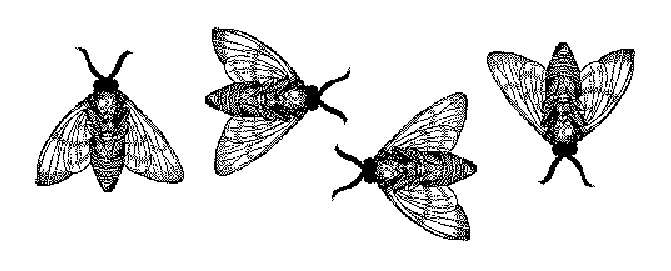
\includegraphics{flies}
\caption{A sample black and white graphic
that needs to span two columns of text.}
\end{figure*}


\begin{figure}
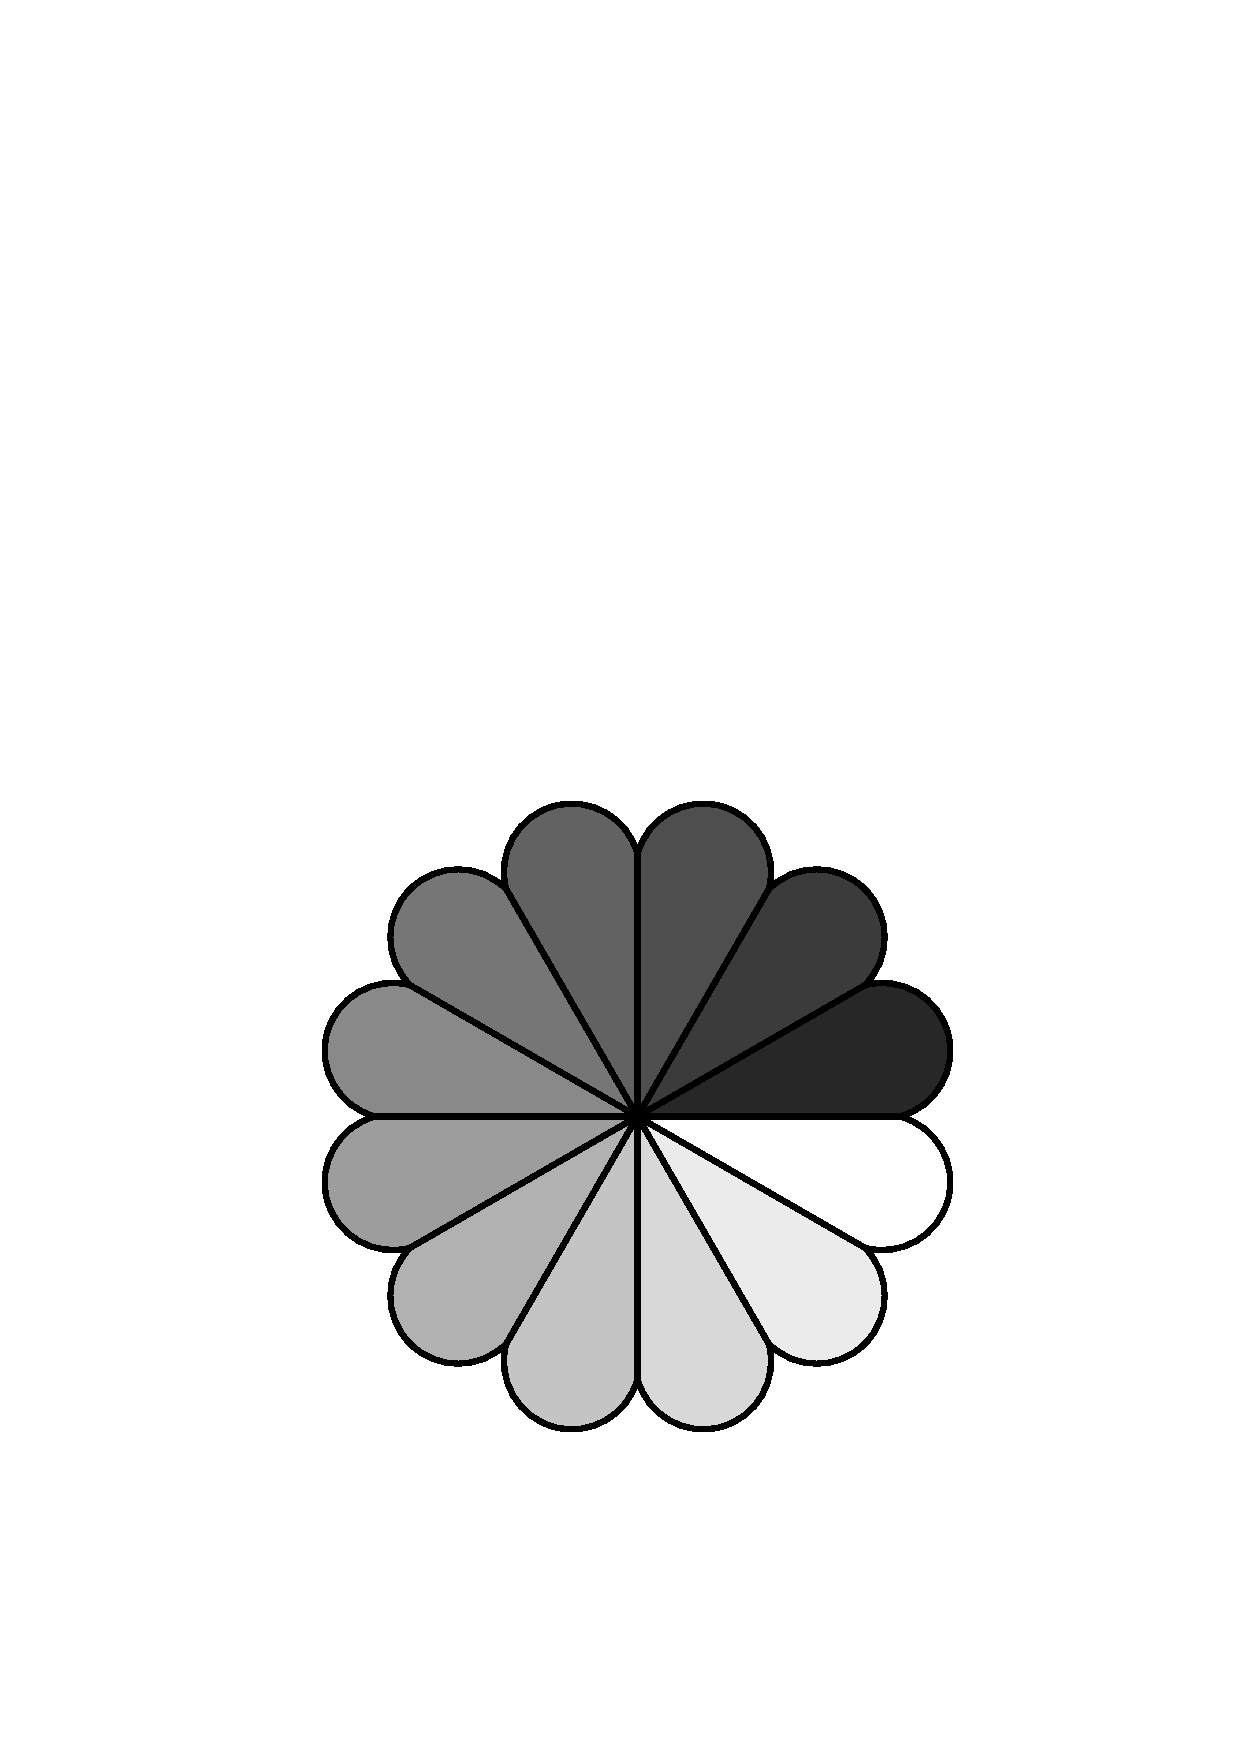
\includegraphics[height=1in, width=1in]{rosette}
\caption{A sample black and white graphic that has
been resized with the \texttt{includegraphics} command.}
\end{figure}

\subsection{Theorem-like Constructs}

Other common constructs that may occur in your article are the forms
for logical constructs like theorems, axioms, corollaries and proofs.
ACM uses two types of these constructs:  theorem-like and
definition-like.

Here is a theorem:
\begin{theorem}
  Let $f$ be continuous on $[a,b]$.  If $G$ is
  an antiderivative for $f$ on $[a,b]$, then
  \begin{displaymath}
    \int^b_af(t)\,dt = G(b) - G(a).
  \end{displaymath}
\end{theorem}

Here is a definition:
\begin{definition}
  If $z$ is irrational, then by $e^z$ we mean the
  unique number that has
  logarithm $z$:
  \begin{displaymath}
    \log e^z = z.
  \end{displaymath}
\end{definition}

The pre-defined theorem-like constructs are \textbf{theorem},
\textbf{conjecture}, \textbf{proposition}, \textbf{lemma} and
\textbf{corollary}.  The pre-defined de\-fi\-ni\-ti\-on-like constructs are
\textbf{example} and \textbf{definition}.  You can add your own
% constructs using the \textsl{amsthm} interface~\cite{Amsthm15}.  The
% styles used in the \verb|\theoremstyle| command are \textbf{acmplain}
% and \textbf{acmdefinition}.

% Another construct is \textbf{proof}, for example,

% \begin{proof}
%   Suppose on the contrary there exists a real number $L$ such that
%   \begin{displaymath}
%     \lim_{x\rightarrow\infty} \frac{f(x)}{g(x)} = L.
  \end{displaymath}
  Then
  \begin{displaymath}
    l=\lim_{x\rightarrow c} f(x)
    = \lim_{x\rightarrow c}
    \left[ g{x} \cdot \frac{f(x)}{g(x)} \right ]
    = \lim_{x\rightarrow c} g(x) \cdot \lim_{x\rightarrow c}
    \frac{f(x)}{g(x)} = 0\cdot L = 0,
  \end{displaymath}
  which contradicts our assumption that $l\neq 0$.
\end{proof}

\section{Conclusions}
This paragraph will end the body of this sample document.
Remember that you might still have Acknowledgments or
Appendices; brief samples of these
follow.  There is still the Bibliography to deal with; and
we will make a disclaimer about that here: with the exception
of the reference to the \LaTeX\ book, the citations in
this paper are to articles which have nothing to
do with the present subject and are used as
examples only.
%\end{document}  % This is where a 'short' article might terminate

\end{comment}
